\documentclass{beamer}
\usepackage{graphicx}
\usepackage{array}
\usepackage{enumitem}  
\graphicspath{ {./img/} }
\usetheme{Warsaw}
\usepackage{polski}
\usepackage[utf8]{inputenc}

\newenvironment<>{varblock}[2][.9\textwidth]{%
  \setlength{\textwidth}{#1}
  \begin{actionenv}#3%
    \def\insertblocktitle{#2}%
    \par%
    \usebeamertemplate{block begin}}
  {\par%
    \usebeamertemplate{block end}%
  \end{actionenv}}

\title{Android Studio}
\definecolor{green}{rgb}{.125,.5,.25}
\usecolortheme[named=green]{structure}
\subtitle{Po co? Dlaczego? Co innego?}
\author{Sielańczyk Jakub}
\date{} 

\begin{document}

    \begin{frame}
        \titlepage
        \begin{center} \vspace{-50pt}
            \includegraphics[scale=0.2]{aslogo}
         \end{center}
    \end{frame}

    \begin{frame}
        \title{Historia}
        \author{}
        \date{}
        \subtitle{}
        \titlepage
    \end{frame}

    \begin{frame}[t]{Historia} \vspace{10pt}
        \begin{description}
            \item[$\bullet$ Prezentacja 0.1v]- 16.05.2013 - Konwerencja Google
            \item[$\bullet$ Pierwsza stabilna wersja] - 01.12.2014
            \item[$\bullet$ Wersja Javy] - ?
            \item[$\bullet$ Wspierane API] - 21
          \end{description}
          \begin{center}
             \includegraphics[scale=0.15]{androidStudioWebsite}
          \end{center}
    \end{frame}

    \begin{frame}[t]{API?} \vspace{10pt}
      \begin{block}{Czym jest API?}
        Android ma kilka ustawień poziomu interfejsu API systemu Android, 
        które określają zgodność aplikacji z wieloma wersjami systemu Android
    \end{block}
        \begin{center}
           \includegraphics[scale=0.2]{api}
        \end{center}
  \end{frame}

    \begin{frame}
        \title{Skład Android Studio}
        \author{}
        \date{}
        \subtitle{}
        \titlepage
    \end{frame}

    \begin{frame}[t]{Skład Android Studio (skrócony)}
          \begin{description}
            \item[$\bullet$ SDK]- Android Software Development Kit
            \item[$\bullet$ NDK]- Android Native Development Kit
            \item[$\bullet$ ADB]- Android Debug Bridge  
            \item[$\bullet$ AVD]- Android Virtual Device
            \item[$\bullet$ Layout Editor]- Simple XML editor
            \item[$\bullet$ Gradle]- Build system   
            \item[$\bullet$ IntelliJ IDEA]- Baza Android Studio
            \item[$\bullet$ Profiler]- Measure app performance
          \end{description}
          \begin{center}
            \includegraphics[scale=0.2]{aslogo}
          \end{center}
    \end{frame}

    \begin{frame}[t]{Android Software Development Kit} 
        \begin{block}{Czym jest SDK?}
            Zestaw narzędzi dla programistów przeznaczony do tworzenia aplikacji na platformę Android. 
            Składa się z dwóch części: 
            \newline SDK Tools – Część wymagana do tworzenia aplikacji niezależnie od wersji Androida
            \newline Platform Tools – Narzędzia zmodyfikowane pod kątem konkretnej wersji systemu
        \end{block}

        \begin{center}\vspace{0pt}
            \includegraphics[scale=0.3]{sdkLogo}
          \end{center}

    \end{frame}

    \begin{frame}[t]{Android Native Development Kit} 
        \begin{block}{Czym jest NDK?}
        Zestaw narzędzi, który umożliwia implementowanie części aplikacji 
            w kodzie natywnym przy użyciu języków takich jak C i C ++ 
  \end{block}
        \begin{center}\vspace{0pt}
            \includegraphics[scale=0.3]{Android-NDK}
          \end{center}

    \end{frame}

    \begin{frame}[t]{Android Debug Bridge} 
        \begin{block}{Czym jest ADB?}
            Wszechstronne narzędzie wiersza poleceń, 
            które umożliwia komunikację z urządzeniem. 
            Polecenie adb ułatwia różne działania na urządzeniu, 
            takie jak instalowanie i debugowanie aplikacji, a także zapewnia dostęp do powłoki systemu Unix, 
            której można używać do uruchamiania różnych poleceń na urządzeniu.  
  \end{block}
        \begin{center}\vspace{0pt}
            \includegraphics[scale=0.5]{adbLogo}
          \end{center}
    \end{frame}

    \begin{frame}[t]{Android Virtual Device} 
        \begin{block}{Czym jest AVD?}
            Urządzenie wirtualne z systemem Android to konfiguracja, 
            która definiuje cechy telefonu, tabletu, Wear OS, Android TV lub Automotive OS 
            urządzenia z systemem Android, które chcesz zasymulować w emulatorze Androida
  \end{block}
        \begin{center}\vspace{0pt}
            \includegraphics[scale=0.3]{avdd}
          \end{center}

        \begin{block}{Ciekawostka}\vspace{-2pt}
            Emulator wykorzystywany przez AVD to qemu 
  \end{block}
    \end{frame}

    \begin{frame}[t]{Layout Editor} 
        \begin{block}{Czym jest Layout Editor?}
            Narzędzie ułatwiające pracę z XML. Domyślnie umożliwia pisanie / tworzenie layuty dynamicznie na wiele platform naraz 
            (Tablety, telefony itd)
            \newline Layout możemy tworzyć w sposób graficzny, tzn przeciągać różne elementy na fragment lub w pełni pisać wszystko ręcznie w XML
            \end{block}
        \begin{center}
            \includegraphics[scale=0.1]{layoutEditor.png}
          \end{center}
    \end{frame}

    \begin{frame}[t]{Gradle} 
        \begin{block}{Czym jest Gradle?}
            Narzędzie do automatyzacji kompilacji oprogramowania 
            w wielu językach na wiele platform. 
            Kontroluje procesy w zadaniach kompilacji, wdrażania i publikowania.
                   \end{block}
        \begin{center}
            \includegraphics[scale=1.0]{gradle.png}
          \end{center}
    \end{frame}

    \begin{frame}[t]{Profiler} 
        \begin{block}{Czym jest Profiler?}
            Narzędzia to, zapewniają dane w czasie rzeczywistym, które pomagają zrozumieć, 
            w jaki sposób aplikacja wykorzystuje zasoby procesora, pamięci, sieci i baterii 
        \end{block}
        \begin{center}
            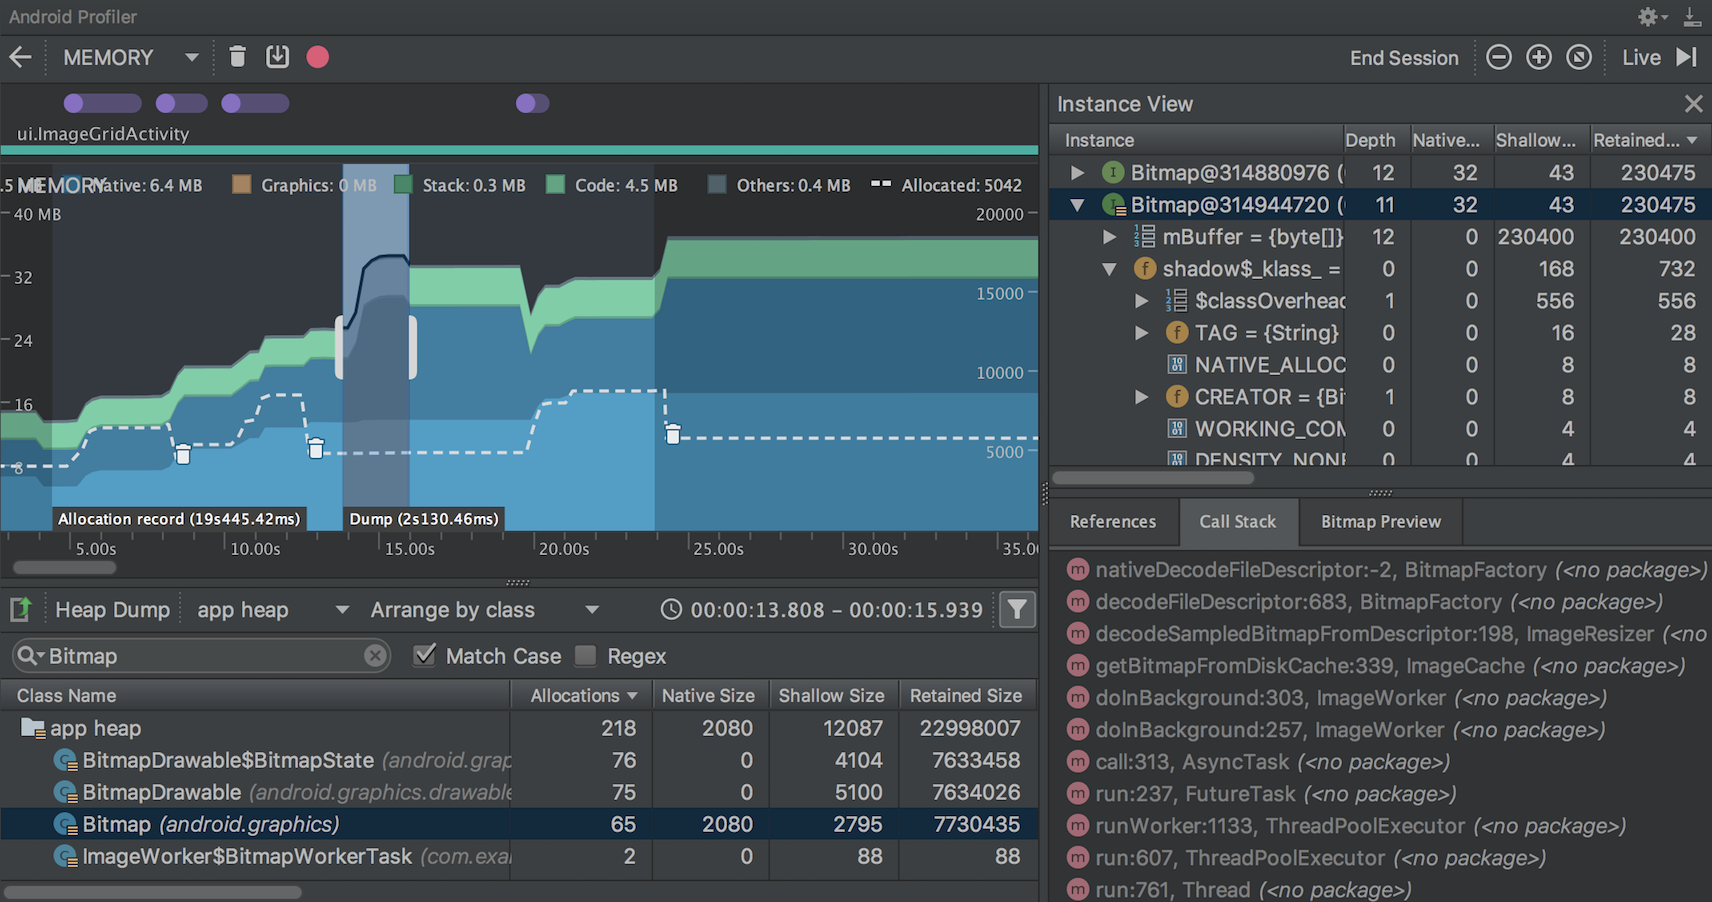
\includegraphics[scale=0.35]{profiler.png}
          \end{center}
    \end{frame}

    \begin{frame}
      \title{Zalety i wady}
      \author{}
      \date{}
      \subtitle{}
      \titlepage
  \end{frame}

  \begin{frame}[t]{Zalety} 
    \begin{description}
      \item[$\bullet$ Cena]- AS jest darmowe. Publikacja aplikacji w oficjalnym sklepie jest jednorazowo płatna
      \item[$\bullet$ All in one]- Wszystko co potrzebne już jest, a mamy nawet wiecej
      \item[$\bullet$ Prostota przygotowawcza]- Instalacja czy konfiguracja to parę kliknięć 
      \item[$\bullet$ Multiplatformowość]- AS natywnie pracuje na systemach \newline Linux / MacOS / Windows
      \item[$\bullet$ Stabilność]- AS naprawdę ciężko zawiesić czy zepsuć
      \item[$\bullet$ Natywne wsparcie Androida]
      \item[$\bullet$ Oficjalne wsparcie Google]
      \item[$\bullet$ Wymagania]- są stosunkowo małe, ale..
    \end{description}
\end{frame}

\definecolor{red}{RGB}{255, 0, 0}
\setbeamercolor{frametitle}{bg=red}
\begin{frame}[t]{Wady} 
  \begin{description}
    \item[$\bullet$ Wymagania]- AS jest jak Chrome. Ile Ramu jest, tyle weźmie
    \item[$\bullet$ Cache]- AS ma z tym niesamowicie duży problem
    \item[$\bullet$ Praca na Windowsie]- Jest zaskakująco gorsza niż na Linuxie czy MacOS 
    \item[$\bullet$ Podfoldery]- Np layouty nie da się rozdzielić na podfoldery
    \item[$\bullet$ Stabilność]- Kiedy się zatnie, nie zawsze to widać
  \end{description}
\end{frame}

\begin{frame}
  \title{Jakaś alternatywa?}
  \author{}
  \date{}
  \subtitle{}
  \titlepage
\end{frame}

\setbeamercolor{frametitle}{bg=green}

\begin{frame}[t]{Eclipse} 
  \begin{center}
    \includegraphics[width=\columnwidth]{eclipse.jpg}
  \end{center}
\end{frame}

\begin{frame}[t]{Xamarin} 
  \begin{center}
    \includegraphics[width=\columnwidth]{Xamarin}
  \end{center}
\end{frame}

\begin{frame}[t]{Koniec} 
  \begin{center}
    \includegraphics[scale=0.4]{aslogo.png}
  \end{center}
\end{frame}

\end{document}

